\documentclass[10pt]{article}

\usepackage[pdftex]{graphicx}% Adds the ability to include images 
\usepackage[margin=2.5cm, top=1cm, a4paper]{geometry}
\usepackage[T1]    {fontenc }% Allow accented output charachters
\usepackage[utf8]  {inputenc}% Allow accented input charachters 
\usepackage    {xcolor   }% Colors are fun :)
\usepackage{array}
\usepackage        {lmodern }% Modern output font 
\usepackage{amsmath,amssymb,latexsym}
\usepackage{fancyhdr}
\setlength{\headheight}{20pt}
\usepackage{sectsty}
\usepackage{hyperref} 
\usepackage{dashrule}
\usepackage{graphicx}

\definecolor{lightgray}{gray}{0.8}

\newcolumntype{L}{>{\raggedleft}p{0.14\textwidth}}
\newcolumntype{R}{p{0.8\textwidth}}
\newcommand\VRule{\color{lightgray}\vrule width 0.5pt}

\pagestyle{fancy}
\fancyhead{}
\fancyfoot{}
\fancyfoot[C]{\emph{Bernát Gábor}\\\thepage}
\fancyfoot[RO, L] {gaborjbernat@gmail.com}
\fancyfoot[LO, R] {$+1$--$747$--$777$--$0357$}
\renewcommand{\headrulewidth}{0pt}

\sectionfont{\fontsize{12}{15}\selectfont}
\newcolumntype{P}[1]{>{\raggedleft\arraybackslash}m{#1}}

\newcommand{\twoColumns}[2]{
  \noindent\begin{tabular}{ p{31em}  P{12.5em} }
    #2 & \emph{#1} \\
\end{tabular}
}
\newcommand{\localsep}{\noindent\hdashrule[0.5ex]{46em}{1pt}{4pt}}

\begin{document}

\begin{minipage}{0.65\textwidth}
	\begin{center}
		\textbf{\Huge{\MakeUppercase{Bernát Gábor}}}\\
		\baselineskip=0pt
		\begin{alignat*}{100}
			\mbox{+}44\mbox{--}79\mbox{--}1997\mbox{--}0265 \mbox{\hspace{0.1cm}} & \Diamond \mbox{\hspace{0.1cm}gaborjbernat@gmail.com} \\
			\mbox{https://bernat.tech} \mbox{\hspace{0.1cm}}                      & \Diamond \mbox{\hspace{0.1cm}Los Angeles, USA}
		\end{alignat*}
	\end{center}
\end{minipage}
\begin{minipage}{0.25\textwidth}
	\flushright{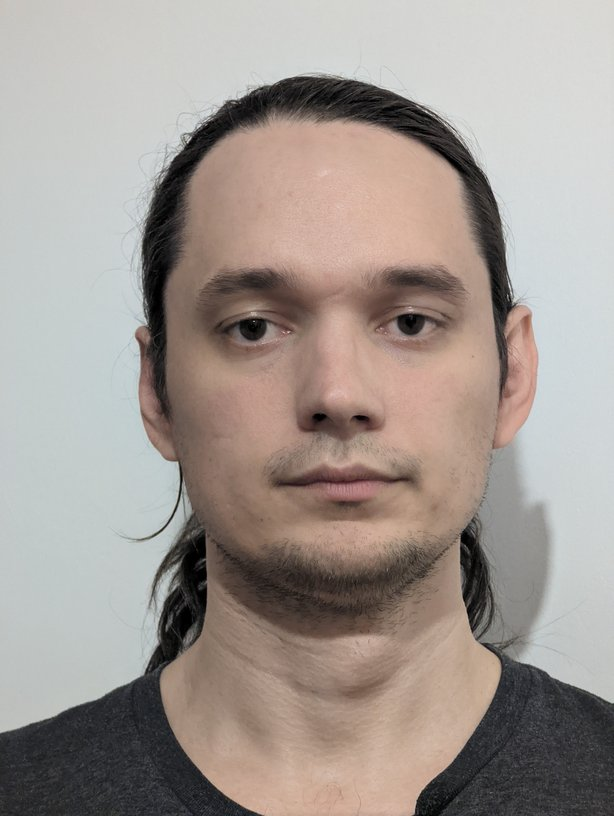
\includegraphics[width=2.5cm]{img/foto.jpeg}}
\end{minipage}

\section*{\MakeUppercase{Summary}}
\leaders\vrule width \textwidth\vskip0.3pt % or other desired thickness
\vskip\medskipamount %

Bernát (first name) Gábor (surname) is a senior software engineer who believes in polyglot
programming (though lately heavily focuses on Python). Currently working full time in Los Angeles at Bloomberg.
He focuses on adding a quality control layer on the data ingestion pipeline built on top of a microservice framework
and generate metrics on how the entire pipeline performs to drive financial analysts day to day work on how they can
improve the non-stock exchange data onboarding for the company.
He finished his master studies in $2013$ with outstanding results in the domain of computer science.


He is a regular Python conference speaker, and authored/maintains many high-profile Python libraries and tools.
He is primaraly focused on packaging and testing (virtualenv, tox, pipx, pipdeptree, build). He is also a conscientious, self-driven
learner and performer, having written multiple successful technical articles on his blog.

\section*{\MakeUppercase{Experience}}
\leaders\vrule width \textwidth\vskip0.3pt % or other desired thickness
\vskip\medskipamount %

\twoColumns{2015--present}{ \textbf{Open Source} }
\twoColumns{Los Angeles, USA}{ \emph{Open source software developer} }

Authored and maintains 20+ Python open source libraries or tools; for a list of high-profile examples see
https://bernat.tech/about. Maintainer of the virtualenv package since 2018. Rewrote and re-released it with success in 2020.
Maintainer of the tox tool since 2017 and close to finishing a rewrite of it. Other high-profile projects he maintains/authored: pipx,
build, filelock, platformdirs, pipdeptree, pytest-env. Regular speaker at the EuroPython and PyCon US conferences (list of recordings at
https://bernat.tech/presentations). Held a workshop about Python packaging at PyCon US 2021.

Received the Python Software Foundation Fellow distinction in 2021 Q3 for outstanding contributions to the Python ecosystem.
Technical reviewer for the book ''Python Object-Oriented Programming 4th edition'' by Steven Lott and Dusty Phillips. Wrote two
blog-post series that made number one on Hackerranks (python type hints and packaging).

\localsep
\vskip\bigskipamount %

\twoColumns{2022 June -- present}{ \textbf{Bloomberg} }
\twoColumns{Los Angeles, USA}{ \emph{Senior Software Engineer} }

Works on the Data Technology department's quality control team on creating a sampling pipeline, extend the departments
metric calculation with dimmensions such as timeliness, remediation and better scalability. Extend the departments tracing functionality
with subtrees. Lead the Python Guilds packaging working group and create a website to help discoverability and ease of contributions
within the company.

\localsep
\vskip\bigskipamount %

\twoColumns{2016 April--2022 June}{ \textbf{Bloomberg} }
\twoColumns{London, United Kingdom}{ \emph{Senior Software Engineer} }

Works on the Data Technology department's quality control team. Responsible for designing and implementing a Python library/framework
that allows financial analysts with limited computer-science knowledge (think simple Python scripting) to express heuristic rules
(ones we can describe - type, range, relations etc.) and semi-automatic rules (i.e. using historical values with statistical models).
The system runs over a microservice framework (think Amazon Lambda) and automatically collects and tracks metadata in the
background which allows answering provenance and data ingestion questions (e.g. what rule checked this field,
how often is this rule broken, validation coverage and efficacy of the pipeline).

Designs and implements a system that calculates metrics about the quality of the data ingestion pipeline and the dataset itself.
Works with other teams to come up with schemas for information to track and then on adoption of those by various
systems in the pipeline. Gives presentations at internal meetups and holds workshops about how to use the quality check system.

Member of the Python Guild Chairs: a group of around 10 engineers fostering the usage and best-practices of the Python language
within the company. Chaired the conference working group since 2018. Maintainer of many high-profile internal tools: one that automatically
generates type information from schemas, HTTP client against a proprietary protocol,  Python abstraction over a service that allows access
of securities, Jenkins CI pipeline library etcetera.

\localsep
\vskip\bigskipamount %

\twoColumns{2011 September--2016 March}{ \textbf{Gravity Research \& Development} }
\twoColumns{Budapest, Hungary}{ \emph{Software and Integration Engineer} }

The company provides hundreds of millions recommendation on a Software--as--a--Service platform
on a daily basis to clients such as dailymotion\@.com, livejasmin\@.com, allegro\@.pl,
edigital\@.hu etcetera. Analyzing customer systems; planning, designing and implementing the
integration of them with the recommendation platform. Performing various AB tests and improvements
after the integration to achieve optimal results, and maximize customer satisfaction. Continuously
keep in touch with customers for fast and accurate feedback on current satisfaction and requirements.

Planning and implementing various internal systems to help with the integration flow and customer
experience (bash shell \& python scripts, PHP \& JavaScript based reporting web page). Programming
and maintaining a recommendation engine demo application (\@.NET \& Silverlight). Transforming the
old and hard-to-modify Ant build system to Gradle. Extending the core system with various new features.
Participating in various conferences to keep up to date with industry trends. Taking part in the hiring
process for new integration engineers, training them and functioning as mentor to them.

\localsep
\vskip\bigskipamount %

\twoColumns{2011 May--August}{ \textbf{OpenCV (Open Source Computer Vision Library)} }
\twoColumns{Târgu Mureş, Romania}{ \emph{Technical writer and programmer (part of Google Summer of Code 2011)} }

Learned and used the reStructuredText documentation system to create various tutorials for the OpenCV
library in both HTML and PDF output format. Helping to architect and create the system used for the
documentation, as well co-supervisoring another person on the project. You can view the end result here:
\emph{http://docs.opencv.org/doc/tutorials/tutorials.html}.

\localsep

\section*{\MakeUppercase{Education}}
\leaders\vrule width \textwidth\vskip0.3pt % or other desired thickness
\vskip\medskipamount %

\twoColumns{2011 September--2013 June}{ \textbf{Budapest University of Technology and Economics, Hungary.} }
\twoColumns{}{Master's degree in Engineering Information Technologist. }

Major in \emph{applied informatics} (grade $4.57/5$ -- excellent). Thesis: "Analysis of data mining and
recommendation services: open source solutions on a scalable framework".

\localsep

\twoColumns{2007 September--2011 June}{ \textbf{Sapientia -- Hungarian University of Transylvania, Romania.} }
\twoColumns{}{Bachelor's degree in Computer Science (grade $9.70/10$).}

Thesis: "Regional segmentation of images with B--Spline level set models".

\section*{\MakeUppercase{Technical strengths}}
\leaders\vrule width \textwidth\vskip0.3pt % or other desired thickness
\vskip\medskipamount %

\begin{tabular}{l p{32em}}
	\textbf{Computer languages} & C/C$++$, C\#, \emph{Java}, Groovy, \emph{Python}, Bash, JavaScript, TypeScript, CSS, HTML, LaTex, reStructuredText, PHP \\
	\textbf{Protocols and apis} & XML, JSON, REST, BAS, jQuery, Qt, SqlAlchemy, JsonRpc, ggplot                                                           \\
	\textbf{Databases}          & comdb2, MySQL (Percona), basic of Cassandra, Hadoop (Hive), Redis                                                       \\
	\textbf{Tools}              & git, vim, tmux, Gradle, Arch Linux, Eclipse, Netbeans, Intellij IDEA, Visual Studio Code, Maven, Gradle,
	Jupyter, tox, JIRA, Confluence                                                                                                                        \\
\end{tabular}
\end{document}
